\documentclass{beamer}
\usepackage{amsmath, amssymb}
\usepackage{physics}
\usepackage{subfig}
\usepackage{hyperref}

\usepackage[utf8]{inputenc}
\usetheme{Madrid}

\title{Usage of JEWEL generator}
\author{Jinghong Yang}

\begin{document}

\begin{frame}
\titlepage
\end{frame}

\begin{frame}
\frametitle{Table of Contents}
\tableofcontents
\end{frame}

\section{Installation}
\begin{frame}
 \frametitle{Installing prerequisites}

 \begin{figure}[h]
  \centering
  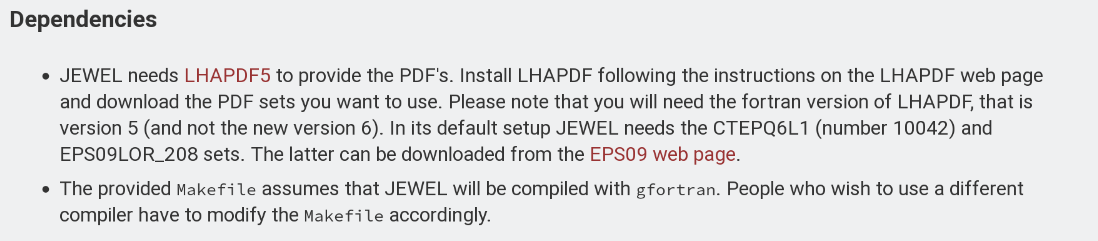
\includegraphics[width=0.9\linewidth]{dependencies.png}
 \end{figure}

 \begin{block}{Download and Install LHAPDF5}
 \begin{scriptsize}
  \url{https://lhapdf.hepforge.org/downloads?f=old}
  \url{https://lhapdf.hepforge.org/lhapdf5/install}
  \end{scriptsize}
 \end{block}

 \begin{block}{\href{https://lhapdf.hepforge.org/lhapdf5/manual\#tth_sEcA}{Download PDF sets} }
 \begin{scriptsize}
  \url{https://lhapdf.hepforge.org/downloads/?f=pdfsets/5.9.1/EPS09LOR_208.LHgrid}
  \url{https://lhapdf.hepforge.org/downloads?f=pdfsets/5.9.1//cteq6ll.LHpdf}
\end{scriptsize}
 \end{block}


\end{frame}

\section{Data generation}

\section{Data processing using RIVET}

\section{Generate gluon and quark jets}

\section{Troubleshooting}

\end{document}


